\PassOptionsToPackage{unicode=true}{hyperref} % options for packages loaded elsewhere
\PassOptionsToPackage{hyphens}{url}
%
\documentclass[]{article}
\usepackage{lmodern}
\usepackage{amssymb,amsmath}
\usepackage{ifxetex,ifluatex}
\usepackage{lscape}
\usepackage{graphicx}
\usepackage{float}
%    \usepackage{lscape}
\usepackage{rotating}
\usepackage{fixltx2e} % provides \textsubscript
\ifnum 0\ifxetex 1\fi\ifluatex 1\fi=0 % if pdftex
  \usepackage[T1]{fontenc}
  \usepackage[utf8]{inputenc}
  \usepackage{textcomp} % provides euro and other symbols
\else % if luatex or xelatex
  \usepackage{unicode-math}
  \defaultfontfeatures{Ligatures=TeX,Scale=MatchLowercase}
\fi
% use upquote if available, for straight quotes in verbatim environments
\IfFileExists{upquote.sty}{\usepackage{upquote}}{}
% use microtype if available
\IfFileExists{microtype.sty}{%
\usepackage[]{microtype}
\UseMicrotypeSet[protrusion]{basicmath} % disable protrusion for tt fonts
}{}
\IfFileExists{parskip.sty}{%
\usepackage{parskip}
}{% else
\setlength{\parindent}{0pt}
\setlength{\parskip}{6pt plus 2pt minus 1pt}
}
\usepackage{hyperref}
\hypersetup{
            pdftitle={arc42 Template},
            pdfborder={0 0 0},
            breaklinks=true}
\urlstyle{same}  % don't use monospace font for urls
\usepackage{longtable,booktabs}
% Fix footnotes in tables (requires footnote package)
\IfFileExists{footnote.sty}{\usepackage{footnote}\makesavenoteenv{longtable}}{}
\usepackage{graphicx,grffile}
\makeatletter
\def\maxwidth{\ifdim\Gin@nat@width>\linewidth\linewidth\else\Gin@nat@width\fi}
\def\maxheight{\ifdim\Gin@nat@height>\textheight\textheight\else\Gin@nat@height\fi}
\makeatother
% Scale images if necessary, so that they will not overflow the page
% margins by default, and it is still possible to overwrite the defaults
% using explicit options in \includegraphics[width, height, ...]{}
\setkeys{Gin}{width=\maxwidth,height=\maxheight,keepaspectratio}
\setlength{\emergencystretch}{3em}  % prevent overfull lines
\providecommand{\tightlist}{%
  \setlength{\itemsep}{0pt}\setlength{\parskip}{0pt}}
\setcounter{secnumdepth}{0}
% Redefines (sub)paragraphs to behave more like sections
\ifx\paragraph\undefined\else
\let\oldparagraph\paragraph
\renewcommand{\paragraph}[1]{\oldparagraph{#1}\mbox{}}
\fi
\ifx\subparagraph\undefined\else
\let\oldsubparagraph\subparagraph
\renewcommand{\subparagraph}[1]{\oldsubparagraph{#1}\mbox{}}
\fi

% set default figure placement to htbp
\makeatletter
\def\fps@figure{htbp}
\makeatother


\title{
\includegraphics{images/arc42-logo.png} Template}
\date{2019-01-04}

\begin{document}
\maketitle

\section{}

\textbf{Über arc42}

arc42, das Template zur Dokumentation von Software- und
Systemarchitekturen.

Erstellt von Dr. Gernot Starke, Dr. Peter Hruschka und Mitwirkenden.

Template Revision: 7.0 DE (asciidoc-based), January 2017

© We acknowledge that this document uses material from the arc42
architecture template, \url{http://www.arc42.de}. Created by Dr. Peter
Hruschka \& Dr. Gernot Starke.

\begin{quote}
\textbf{Note}

Diese Version des Templates enthält Hilfen und Erläuterungen. Sie dient
der Einarbeitung in arc42 sowie dem Verständnis der Konzepte. Für die
Dokumentation eigener System verwenden Sie besser die \emph{plain}
Version.
\end{quote}

\hypertarget{section-introduction-and-goals}{%
\section{Einführung und Ziele}\label{section-introduction-and-goals}}

Beschreibt die wesentlichen Anforderungen und treibenden Kräfte, die bei
der Umsetzung der Softwarearchitektur und Entwicklung des Systems
berücksichtigt werden müssen.

Dazu gehören:

\begin{itemize}
\item
  zugrunde liegende Geschäftsziele,
\item
  wesentliche Aufgabenstellungen und
\item
  essenzielle fachliche Anforderungen an das System sowie
\item
  Qualitätsziele für die Architektur und
\item
  relevante Stakeholder und deren Erwartungshaltung.
\end{itemize}

\hypertarget{_aufgabenstellung}{%
\subsection{Aufgabenstellung}\label{_aufgabenstellung}}

\textbf{Inhalt.}

Kurzbeschreibung der fachlichen Aufgabenstellung, treibenden Kräfte,
Extrakt (oder Abstract) der Anforderungen. Verweis auf (hoffentlich
vorliegende) Anforderungsdokumente (mit Versionsbezeichnungen und
Ablageorten).

\textbf{Motivation.}

Aus Sicht der späteren Nutzung ist die Unterstützung einer fachlichen
Aufgabe oder Verbesserung der Qualität der eigentliche Beweggrund, ein
neues System zu schaffen oder ein bestehendes zu modifizieren.

\textbf{Form.}

Kurze textuelle Beschreibung, eventuell in tabellarischer Use-Case Form.
Sofern vorhanden, sollte die Aufgabenstellung Verweise auf die
entsprechenden Anforderungsdokumente enthalten.

Halten Sie diese Auszüge so knapp wie möglich und wägen Sie Lesbarkeit
und Redundanzfreiheit gegeneinander ab.

\hypertarget{_qualit_tsziele}{%
\subsection{Qualitätsziele}\label{_qualit_tsziele}}

\textbf{Inhalt.}

Die Top-3 bis Top-5 der Qualitätsziele für die Architektur, deren
Erfüllung oder Einhaltung den maßgeblichen Stakeholdern besonders
wichtig sind. Gemeint sind hier wirklich Qualitätsziele, die nicht
unbedingt mit den Zielen des Projekts übereinstimmen. Beachten Sie den
Unterschied.

\textbf{Motivation.}

Weil Qualitätsziele grundlegende Architekturentscheidungen oft
maßgeblich beeinflussen, sollten Sie die für Ihre Stakeholder relevanten
Qualitätsziele kennen, möglichst konkret und operationalisierbar.

\textbf{Form.}

Tabellarische Darstellung der Qualitätsziele mit möglichst konkreten
Szenarien, geordnet nach Prioritäten.

\hypertarget{_stakeholder}{%
\subsection{Stakeholder}\label{_stakeholder}}

\begin{longtable}[]{@{}lll@{}}
\toprule
\begin{minipage}[b]{0.23\columnwidth}\raggedright
Rolle\strut
\end{minipage} & \begin{minipage}[b]{0.23\columnwidth}\raggedright
Kontakt\strut
\end{minipage} & \begin{minipage}[b]{0.46\columnwidth}\raggedright
Erwartungshaltung\strut
\end{minipage}\tabularnewline
\midrule
\endhead
\begin{minipage}[t]{0.23\columnwidth}\raggedright
	\emph{CEO}\strut
\end{minipage} & \begin{minipage}[t]{0.23\columnwidth}\raggedright
\emph{Dr. Michael Moore}\strut
\end{minipage} & \begin{minipage}[t]{0.46\columnwidth}\raggedright
\emph{Keine Vollautomatisierung, Segnet alle Boni manuell ab}\strut
\end{minipage}\tabularnewline
\begin{minipage}[t]{0.23\columnwidth}\raggedright
\emph{HR Senior Consultant}\strut
\end{minipage} & \begin{minipage}[t]{0.23\columnwidth}\raggedright
\emph{Chantal Banks}\strut
\end{minipage} & \begin{minipage}[t]{0.46\columnwidth}\raggedright
\emph{Weniger manuelle Schritte, Keine Papierarbeit mehr}\strut
\end{minipage}\tabularnewline
\begin{minipage}[t]{0.23\columnwidth}\raggedright
	\emph{IT-Admin}\strut
\end{minipage} & \begin{minipage}[t]{0.23\columnwidth}\raggedright
	\emph{Tom Foster}\strut
\end{minipage} & \begin{minipage}[t]{0.46\columnwidth}\raggedright
	\emph{Keine Berührungspunkte mit dem gesamten Prozess}\strut
\end{minipage}\tabularnewline
\bottomrule
\end{longtable}


\hypertarget{section-architecture-constraints}{%
\section{Randbedingungen}\label{section-architecture-constraints}}

\textbf{Inhalt.}

Beschreibung der zu nutzenden externen Systemen

\textbf{Was ist die prinzipielle Aufgabe der Anwendung OpenCRX? }
\begin{itemize}
\item CRM System
\item Account management
\item Product and Price Management
\item Sales Pipeline
\item Issue tracking
\item Groupware
\item mail, contact and calendar management
\end{itemize}

\textbf{Was ist die prinzipielle Aufgabe der Anwendung OrangeHRM? }
\begin{itemize}
	\item an Resource Management
	\item mance Management
	\item  Administration and Personal Information Management
	\item  Recruitment etc.
	\item  Employee Self Service (Time Tracking)
\end{itemize}

\textbf{Welche grundlegenden Funktionen besitzen diese Anwendungen?}
OrangeHRM bietet Funktionalitäten zum Verwalten des Personals und alles was dazu gehört:
\begin{itemize}
	\item Mitarbeiterverwaltung inkl. Mitarbeiter Self Service
	\item Dashboards
	\item Mitarbeiter Training
	\item Reiseplanung
	\item Dokumentenmanager
	\item OpenCRX bietet Funktionalitäten zur Verwaltung von Kunden
	\item Kundensupport
	\item Customer Success
	\item Marketing
	\item Analytics
	\item Sales Management
\end{itemize}

\textbf{Welche Geschäftsobjekte werden in OpenCRX bzw. OrangeHRM verwaltet?}
\begin{itemize}
	\item Kunden
	\item Mitarbeiter
\end{itemize}
\textbf{Welche Art Schnittstellen bieten OpenCRX bzw. OrangeHRM an?}
	\begin{itemize}
	\item OpenCRX:
	\begin{itemize}
		\item REST API
		\item AirSync ActiveSync
		\item User Interface (WebUI)
	\end{itemize}
	\item OrangeHRM:
		\begin{itemize}
			\item REST API
			\item Mobile APP
			\item User Interface (WebUI)
		\end{itemize}
\end{itemize}


\hypertarget{section-system-scope-and-context}{%
\section{Kontextabgrenzung}\label{section-system-scope-and-context}}

\textbf{Inhalt.}

Die Kontextabgrenzung grenzt das System von allen
Kommunikationsbeziehungen (Nachbarsystemen und Benutzerrollen) ab. Sie
legt damit die externen Schnittstellen fest.

Differenzieren Sie fachliche (fachliche Ein- und Ausgaben) und
technische Kontexte (Kanäle, Protokolle, Hardware), falls nötig.

\textbf{Motivation.}

Die fachlichen und technischen Schnittstellen zur Kommunikation gehören
zu den kritischsten Aspekten eines Systems. Stellen Sie sicher, dass Sie
diese komplett verstanden haben.

\textbf{Form.}

Verschiedene Optionen:

\begin{itemize}
\item
  Diverse Kontextdiagramme
\item
  Listen von Kommunikationsbeziehungen mit deren Schnittstellen
\end{itemize}

\hypertarget{_fachlicher_kontext}{%
\subsection{Fachlicher Kontext}\label{_fachlicher_kontext}}

\textbf{Inhalt.}

Festlegung \textbf{aller} Kommunikationsbeziehungen (Nutzer, IT-Systeme,
\ldots{}) mit Erklärung der fachlichen Ein- und Ausgabedaten oder
Schnittstellen. Zusätzlich (bei Bedarf) fachliche Datenformate oder
Protokolle der Kommunikation mit den Nachbarsystemen.

\textbf{Motivation.}

Alle Beteiligten müssen verstehen, welche fachlichen Informationen mit
der Umwelt ausgetauscht werden.

\textbf{Lösung}

\begin{figure}[H]
	\centering
	\includegraphics[width=1.0\linewidth]{"images/uebung6_4_kontext_sicht"}
	\caption{Fachlicher Kontext}
	\label{fig:uebung64kontextsicht}
\end{figure}


\textbf{\textless{}optional: Erläuterung der externen fachlichen
Schnittstellen\textgreater{}}


\hypertarget{_technischer_kontext}{%
\subsection{Technischer Kontext}\label{_technischer_kontext}}

\textbf{Inhalt.}

Technische Schnittstellen (Kanäle, Übertragungsmedien) zwischen dem
System und seiner Umwelt. Zusätzlich eine Erklärung (\emph{mapping}),
welche fachlichen Ein- und Ausgaben über welche technischen Kanäle
fließen.

\textbf{Motivation.}

Viele Stakeholder treffen Architekturentscheidungen auf Basis der
technischen Schnittstellen des Systems zu seinem Kontext.

Insbesondere bei der Entwicklung von Infrastruktur oder Hardware sind
diese technischen Schnittstellen durchaus entscheidend.

\textbf{Form.}

Beispielsweise UML Deployment-Diagramme mit den Kanälen zu
Nachbarsystemen, begleitet von einer Tabelle, die Kanäle auf
Ein-/Ausgaben abbildet.

\textbf{Lösung}


\textbf{\textless{}Mapping fachliche auf technische
Schnittstellen\textgreater{}}

\hypertarget{section-solution-strategy}{%
\section{Lösungsstrategie}\label{section-solution-strategy}}

\textbf{Inhalt.}

Kurzer Überblick über die grundlegenden Entscheidungen und
Lösungsansätze, die Entwurf und Implementierung des Systems prägen.
Hierzu gehören:

\begin{itemize}
\item
  Technologieentscheidungen
\item
  Entscheidungen über die Top-Level-Zerlegung des Systems,
  beispielsweise die Verwendung gesamthaft prägender Entwurfs- oder
  Architekturmuster,
\item
  Entscheidungen zur Erreichung der wichtigsten Qualitätsanforderungen
  sowie
\item
  relevante organisatorische Entscheidungen, beispielsweise für
  bestimmte Entwicklungsprozesse oder Delegation bestimmter Aufgaben an
  andere Stakeholder.
\end{itemize}

\textbf{Motivation.}

Diese wichtigen Entscheidungen bilden wesentliche „Eckpfeiler`` der
Architektur. Von ihnen hängen viele weitere Entscheidungen oder
Implementierungsregeln ab.

\textbf{Form.}

Fassen Sie die zentralen Entwurfsentscheidungen \textbf{kurz} zusammen.
Motivieren Sie, ausgehend von Aufgabenstellung, Qualitätszielen und
Randbedingungen, was Sie entschieden haben und warum Sie so entschieden
haben. Vermeiden Sie redundante Beschreibungen und verweisen Sie eher
auf weitere Ausführungen in Folgeabschnitten.

\hypertarget{section-building-block-view}{%
\section{Bausteinsicht}\label{section-building-block-view}}

\begin{figure}[H]
	\centering
	\includegraphics[width=1.0\linewidth]{"images/uebung6_4_baustein_sicht"}
	\caption{Bausteinsicht}
	\label{fig:uebung64bausteinsicht}
\end{figure}


\hypertarget{_whitebox_gesamtsystem}{%
\subsection{Whitebox Gesamtsystem}\label{_whitebox_gesamtsystem}}

An dieser Stelle beschreiben Sie die Zerlegung des Gesamtsystems anhand
des nachfolgenden Whitebox-Templates. Dieses enthält:

\begin{itemize}
\item
  Ein Übersichtsdiagramm
\item
  die Begründung dieser Zerlegung
\item
  Blackbox-Beschreibungen der hier enthaltenen Bausteine. Dafür haben
  Sie verschiedene Optionen:

  \begin{itemize}
  \item
    in \emph{einer} Tabelle, gibt einen kurzen und pragmatischen
    Überblick über die enthaltenen Bausteine sowie deren Schnittstellen.
  \item
    als Liste von Blackbox-Beschreibungen der Bausteine, gemäß dem
    Blackbox-Template (siehe unten). Diese Liste können Sie, je nach
    Werkzeug, etwa in Form von Unterkapiteln (Text), Unter-Seiten (Wiki)
    oder geschachtelten Elementen (Modellierungswerkzeug) darstellen.
  \end{itemize}
\item
  (optional:) wichtige Schnittstellen, die nicht bereits im
  Blackbox-Template eines der Bausteine erläutert werden, aber für das
  Verständnis der Whitebox von zentraler Bedeutung sind. Aufgrund der
  vielfältigen Möglichkeiten oder Ausprägungen von Schnittstellen geben
  wir hierzu kein weiteres Template vor. Im schlimmsten Fall müssen Sie
  Syntax, Semantik, Protokolle, Fehlerverhalten, Restriktionen,
  Versionen, Qualitätseigenschaften, notwendige Kompatibilitäten und
  vieles mehr spezifizieren oder beschreiben. Im besten Fall kommen Sie
  mit Beispielen oder einfachen Signaturen zurecht.
\end{itemize}

\emph{\textbf{\textless{}Übersichtsdiagramm\textgreater{}}}

\begin{description}
\item[Begründung]
\emph{\textless{}Erläuternder Text\textgreater{}}
\item[Enthaltene Bausteine]
\emph{\textless{}Beschreibung der enthaltenen Bausteine
(Blackboxen)\textgreater{}}
\item[Wichtige Schnittstellen]
\emph{\textless{}Beschreibung wichtiger Schnittstellen\textgreater{}}
\end{description}

Hier folgen jetzt Erläuterungen zu Blackboxen der Ebene 1.

Falls Sie die tabellarische Beschreibung wählen, so werden Blackboxen
darin nur mit Name und Verantwortung nach folgendem Muster beschrieben:

\begin{longtable}[]{@{}ll@{}}
\toprule
\begin{minipage}[b]{0.31\columnwidth}\raggedright
\textbf{Name}\strut
\end{minipage} & \begin{minipage}[b]{0.63\columnwidth}\raggedright
\textbf{Verantwortung}\strut
\end{minipage}\tabularnewline
\midrule
\endhead
\begin{minipage}[t]{0.31\columnwidth}\raggedright
\emph{\textless{}Blackbox 1\textgreater{}}\strut
\end{minipage} & \begin{minipage}[t]{0.63\columnwidth}\raggedright
~\emph{\textless{}Text\textgreater{}}\strut
\end{minipage}\tabularnewline
\begin{minipage}[t]{0.31\columnwidth}\raggedright
\emph{\textless{}Blackbox 2\textgreater{}}\strut
\end{minipage} & \begin{minipage}[t]{0.63\columnwidth}\raggedright
~\emph{\textless{}Text\textgreater{}}\strut
\end{minipage}\tabularnewline
\bottomrule
\end{longtable}

Falls Sie die ausführliche Liste von Blackbox-Beschreibungen wählen,
beschreiben Sie jede wichtige Blackbox in einem eigenen
Blackbox-Template. Dessen Überschrift ist jeweils der Namen dieser
Blackbox.

\hypertarget{__name_blackbox_1}{%
\subsubsection{\textless{}Name Blackbox
1\textgreater{}}\label{__name_blackbox_1}}

Beschreiben Sie die \textless{}Blackbox 1\textgreater{} anhand des
folgenden Blackbox-Templates:

\begin{itemize}
\item
  Zweck/Verantwortung
\item
  Schnittstelle(n), sofern diese nicht als eigenständige Beschreibungen
  herausgezogen sind. Hierzu gehören eventuell auch Qualitäts- und
  Leistungsmerkmale dieser Schnittstelle.
\item
  (Optional) Qualitäts-/Leistungsmerkmale der Blackbox, beispielsweise
  Verfügbarkeit, Laufzeitverhalten o. Ä.
\item
  (Optional) Ablageort/Datei(en)
\item
  (Optional) Erfüllte Anforderungen, falls Sie Traceability zu
  Anforderungen benötigen.
\item
  (Optional) Offene Punkte/Probleme/Risiken
\end{itemize}

\emph{\textless{}Zweck/Verantwortung\textgreater{}}

\emph{\textless{}Schnittstelle(n)\textgreater{}}

\emph{\textless{}(Optional) Qualitäts-/Leistungsmerkmale\textgreater{}}

\emph{\textless{}(Optional) Ablageort/Datei(en)\textgreater{}}

\emph{\textless{}(Optional) Erfüllte Anforderungen\textgreater{}}

\emph{\textless{}(optional) Offene
Punkte/Probleme/Risiken\textgreater{}}

\hypertarget{__name_blackbox_2}{%
\subsubsection{\textless{}Name Blackbox
2\textgreater{}}\label{__name_blackbox_2}}

\emph{\textless{}Blackbox-Template\textgreater{}}

\hypertarget{__name_blackbox_n}{%
\subsubsection{\textless{}Name Blackbox
n\textgreater{}}\label{__name_blackbox_n}}

\emph{\textless{}Blackbox-Template\textgreater{}}

\hypertarget{__name_schnittstelle_1}{%
\subsubsection{\textless{}Name Schnittstelle
1\textgreater{}}\label{__name_schnittstelle_1}}

\ldots{}

\hypertarget{__name_schnittstelle_m}{%
\subsubsection{\textless{}Name Schnittstelle
m\textgreater{}}\label{__name_schnittstelle_m}}

\hypertarget{_ebene_2}{%
\subsection{Ebene 2}\label{_ebene_2}}

Beschreiben Sie den inneren Aufbau (einiger) Bausteine aus Ebene 1 als
Whitebox.

Welche Bausteine Ihres Systems Sie hier beschreiben, müssen Sie selbst
entscheiden. Bitte stellen Sie dabei Relevanz vor Vollständigkeit.
Skizzieren Sie wichtige, überraschende, riskante, komplexe oder
besonders volatile Bausteine. Normale, einfache oder standardisierte
Teile sollten Sie weglassen.

\hypertarget{_whitebox_emphasis_baustein_1_emphasis}{%
\subsubsection{\texorpdfstring{Whitebox \emph{\textless{}Baustein
1\textgreater{}}}{Whitebox \textless{}Baustein 1\textgreater{}}}\label{_whitebox_emphasis_baustein_1_emphasis}}

\ldots{}zeigt das Innenleben von \emph{Baustein 1}.

\emph{\textless{}Whitebox-Template\textgreater{}}

\hypertarget{_whitebox_emphasis_baustein_2_emphasis}{%
\subsubsection{\texorpdfstring{Whitebox \emph{\textless{}Baustein
2\textgreater{}}}{Whitebox \textless{}Baustein 2\textgreater{}}}\label{_whitebox_emphasis_baustein_2_emphasis}}

\emph{\textless{}Whitebox-Template\textgreater{}}

\ldots{}

\hypertarget{_whitebox_emphasis_baustein_m_emphasis}{%
\subsubsection{\texorpdfstring{Whitebox \emph{\textless{}Baustein
m\textgreater{}}}{Whitebox \textless{}Baustein m\textgreater{}}}\label{_whitebox_emphasis_baustein_m_emphasis}}

\emph{\textless{}Whitebox-Template\textgreater{}}

\hypertarget{_ebene_3}{%
\subsection{Ebene 3}\label{_ebene_3}}

Beschreiben Sie den inneren Aufbau (einiger) Bausteine aus Ebene 2 als
Whitebox.

Bei tieferen Gliederungen der Architektur kopieren Sie diesen Teil von
arc42 für die weiteren Ebenen.

\hypertarget{_whitebox_baustein_x_1}{%
\subsubsection{Whitebox \textless{}\_Baustein
x.1\_\textgreater{}}\label{_whitebox_baustein_x_1}}

\ldots{}zeigt das Innenleben von \emph{Baustein x.1}.

\emph{\textless{}Whitebox-Template\textgreater{}}

\hypertarget{_whitebox_baustein_x_2}{%
\subsubsection{Whitebox \textless{}\_Baustein
x.2\_\textgreater{}}\label{_whitebox_baustein_x_2}}

\emph{\textless{}Whitebox-Template\textgreater{}}

\hypertarget{_whitebox_baustein_y_1}{%
\subsubsection{Whitebox \textless{}\_Baustein
y.1\_\textgreater{}}\label{_whitebox_baustein_y_1}}

\emph{\textless{}Whitebox-Template\textgreater{}}

\hypertarget{section-runtime-view}{\section{Laufzeitsicht}\label{section-runtime-view}}

\begin{figure}[H]
	\centering
	\rotatebox{90}{\includegraphics[width=1.7\linewidth]{"images/laufzeitsicht_high_performance_bpmn"}}
	\caption{Laufzeitsicht}
	\label{fig:laufzeitsichthighperformancebpmn}
\end{figure}


\hypertarget{section-deployment-view}{%
\section{Verteilungssicht}\label{section-deployment-view}}
\begin{figure}[H]
	\centering
	\includegraphics[width=1.0\linewidth]{"images/verteilungssicht"}
	\caption{Verteilungssicht}
	\label{fig:verteilungssicht}
\end{figure}

\hypertarget{_infrastruktur_ebene_1}{%
\subsection{Infrastruktur Ebene 1}\label{_infrastruktur_ebene_1}}

An dieser Stelle beschreiben Sie (als Kombination von Diagrammen mit
Tabellen oder Texten):

\begin{itemize}
\item
  die Verteilung des Gesamtsystems auf mehrere Standorte, Umgebungen,
  Rechner, Prozessoren o. Ä., sowie die physischen Verbindungskanäle
  zwischen diesen,
\item
  wichtige Begründungen für diese Verteilungsstruktur,
\item
  Qualitäts- und/oder Leistungsmerkmale dieser Infrastruktur,
\item
  Zuordnung von Softwareartefakten zu Bestandteilen der Infrastruktur
\end{itemize}

Für mehrere Umgebungen oder alternative Deployments kopieren Sie diesen
Teil von arc42 für alle wichtigen Umgebungen/Varianten.

\emph{\textbf{\textless{}Übersichtsdiagramm\textgreater{}}}

\begin{description}
\item[Begründung]
\emph{\textless{}Erläuternder Text\textgreater{}}
\item[Qualitäts- und/oder Leistungsmerkmale]
\emph{\textless{}Erläuternder Text\textgreater{}}
\item[Zuordnung von Bausteinen zu Infrastruktur]
\emph{\textless{}Beschreibung der Zuordnung\textgreater{}}
\end{description}

\hypertarget{_infrastruktur_ebene_2}{%
\subsection{Infrastruktur Ebene 2}\label{_infrastruktur_ebene_2}}

An dieser Stelle können Sie den inneren Aufbau (einiger)
Infrastrukturelemente aus Ebene 1 beschreiben.

Für jedes Infrastrukturelement kopieren Sie die Struktur aus Ebene 1.

\hypertarget{__emphasis_infrastrukturelement_1_emphasis}{%
\subsubsection{\texorpdfstring{\emph{\textless{}Infrastrukturelement
1\textgreater{}}}{\textless{}Infrastrukturelement 1\textgreater{}}}\label{__emphasis_infrastrukturelement_1_emphasis}}

\emph{\textless{}Diagramm + Erläuterungen\textgreater{}}

\hypertarget{__emphasis_infrastrukturelement_2_emphasis}{%
\subsubsection{\texorpdfstring{\emph{\textless{}Infrastrukturelement
2\textgreater{}}}{\textless{}Infrastrukturelement 2\textgreater{}}}\label{__emphasis_infrastrukturelement_2_emphasis}}

\emph{\textless{}Diagramm + Erläuterungen\textgreater{}}

\ldots{}

\hypertarget{__emphasis_infrastrukturelement_n_emphasis}{%
\subsubsection{\texorpdfstring{\emph{\textless{}Infrastrukturelement
n\textgreater{}}}{\textless{}Infrastrukturelement n\textgreater{}}}\label{__emphasis_infrastrukturelement_n_emphasis}}

\emph{\textless{}Diagramm + Erläuterungen\textgreater{}}

\hypertarget{section-concepts}{%
\section{Querschnittliche Konzepte}\label{section-concepts}}

\textbf{Inhalt.}

Dieser Abschnitt beschreibt übergreifende, prinzipielle Regelungen und
Lösungsansätze, die an mehreren Stellen (=\emph{querschittlich})
relevant sind.

Solche Konzepte betreffen oft mehrere Bausteine. Dazu können vielerlei
Themen gehören, beispielsweise:

\begin{itemize}
\item
  fachliche Modelle,
\item
  eingesetzte Architektur- oder Entwurfsmuster,
\item
  Regeln für den konkreten Einsatz von Technologien,
\item
%  prinzipielle --- meist technische --- Festlegungen übergreifender Art,
\item
  Implementierungsregeln
\end{itemize}

\textbf{Motivation.}

Konzepte bilden die Grundlage für \emph{konzeptionelle Integrität}
(Konsistenz, Homogenität) der Architektur und damit eine wesentliche
Grundlage für die innere Qualität Ihrer Systeme.

Manche dieser Themen lassen sich nur schwer als Baustein in der
Architektur unterbringen (z.B. das Thema „Sicherheit``). Hier ist der
Platz im Template, wo Sie derartige Themen geschlossen behandeln können.

\textbf{Form.}

Kann vielfältig sein:

\begin{itemize}
\item
  Konzeptpapiere mit beliebiger Gliederung,
\item
  übergreifende Modelle/Szenarien mit Notationen, die Sie auch in den
  Architektursichten nutzen,
\item
  beispielhafte Implementierung speziell für technische Konzepte,
\item
  Verweise auf „übliche`` Nutzung von Standard-Frameworks
  (beispielsweise die Nutzung von Hibernate als Object/Relational
  Mapper).
\end{itemize}

\textbf{Struktur.}

Eine mögliche (nicht aber notwendige!) Untergliederung dieses
Abschnittes könnte wie folgt aussehen (wobei die Zuordnung von Themen zu
den Gruppen nicht immer eindeutig ist):

\begin{itemize}
\item
  Fachliche Konzepte
\item
  User Experience (UX)
\item
  Sicherheitskonzepte (Safety und Security)
\item
  Architektur- und Entwurfsmuster
\item
  Unter-der-Haube
\item
  Entwicklungskonzepte
\item
  Betriebskonzepte
\end{itemize}

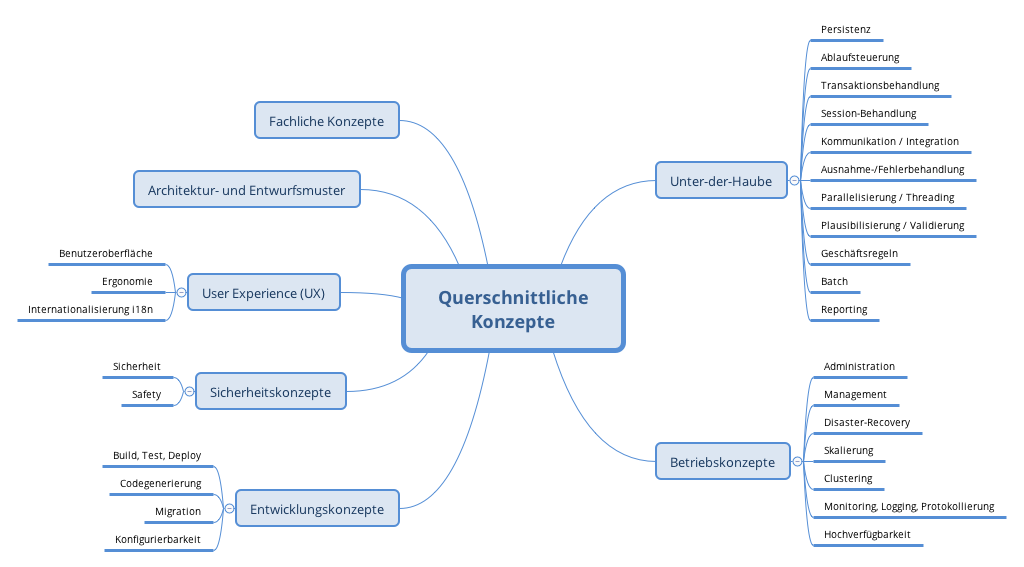
\includegraphics{images/08-Crosscutting-Concepts-Structure-DE.png}

\hypertarget{__emphasis_konzept_1_emphasis}{%
\subsection{\texorpdfstring{\emph{\textless{}Konzept
1\textgreater{}}}{\textless{}Konzept 1\textgreater{}}}\label{__emphasis_konzept_1_emphasis}}

\emph{\textless{}Erklärung\textgreater{}}

\hypertarget{__emphasis_konzept_2_emphasis}{%
\subsection{\texorpdfstring{\emph{\textless{}Konzept
2\textgreater{}}}{\textless{}Konzept 2\textgreater{}}}\label{__emphasis_konzept_2_emphasis}}

\emph{\textless{}Erklärung\textgreater{}}

\ldots{}

\hypertarget{__emphasis_konzept_n_emphasis}{%
\subsection{\texorpdfstring{\emph{\textless{}Konzept
n\textgreater{}}}{\textless{}Konzept n\textgreater{}}}\label{__emphasis_konzept_n_emphasis}}

\emph{\textless{}Erklärung\textgreater{}}

\hypertarget{section-design-decisions}{%
\section{Entwurfsentscheidungen}\label{section-design-decisions}}

Zur prototypischen Implementierung wurden verschiedene Sprachen und Technologien verwendet, welche in diesem Abschnitt erläutert werden.

Wie vorgegeben wurde zur modellierung des Workflows das Tool Camunda eingesetzt. Mithilfe von Camunda wurde der gesamte Prozess modeliert und ausgeführt. Das Camunda Cockpit und die Tasklist eignen sich hervorragend zum starten und verwalten der Prozesse. 
Da im verlaufe des Prozesses auch mit Fremdsystemen kommuniziert werden muss wurde ein Microservice in der Sprache Kotlin entwickelt. Dieser Service übernimmt die Kommunikation mit OrangeHRM und OpenCRX über die dokumentierten REST API's.
Um eine konsistene Architektur bereitzustellen bietet der Microservce ebenfalls REST-Schnittstellen an, welche aus der JavaDelegate Klasse aus Camunda heraus aufgerufen wird. 
Zum vereinfachten deployment des Dienstes wird dieser in einem Docker Container ausgeführt.


\hypertarget{section-technical-risks}{%
\section{Risiken und technische
Schulden}\label{section-technical-risks}}

\textbf{Inhalt.}

Eine nach Prioritäten geordnete Liste der erkannten Architekturrisiken
und/oder technischen Schulden.

\begin{quote}
Risikomanagement ist Projektmanagement für Erwachsene.

---  Tim Lister Atlantic Systems Guild
\end{quote}

Unter diesem Motto sollten Sie Architekturrisiken und/oder technische
Schulden gezielt ermitteln, bewerten und Ihren Management-Stakeholdern
(z.B. Projektleitung, Product-Owner) transparent machen.

\textbf{Form.}

Liste oder Tabelle von Risiken und/oder technischen Schulden, eventuell
mit vorgeschlagenen Maßnahmen zur Risikovermeidung, Risikominimierung
oder dem Abbau der technischen Schulden.

\hypertarget{section-glossary}{%
\section{Glossar}\label{section-glossary}}

\textbf{Inhalt.}

Die wesentlichen fachlichen und technischen Begriffe, die Stakeholder im
Zusammenhang mit dem System verwenden.

Nutzen Sie das Glossar ebenfalls als Übersetzungsreferenz, falls Sie in
mehrsprachigen Teams arbeiten.

\textbf{Motivation.}

Sie sollten relevante Begriffe klar definieren, so dass alle Beteiligten

\begin{enumerate}
\def\labelenumi{\arabic{enumi}.}
\item
  diese Begriffe identisch verstehen, und
\item
  vermeiden, mehrere Begriffe für die gleiche Sache zu haben.
\end{enumerate}

\begin{itemize}
\item
  Zweispaltige Tabelle mit \textless{}Begriff\textgreater{} und
  \textless{}Definition\textgreater{}
\item
  Eventuell weitere Spalten mit Übersetzungen, falls notwendig.
\end{itemize}

\begin{longtable}[]{@{}ll@{}}
\toprule
\begin{minipage}[b]{0.31\columnwidth}\raggedright
Begriff\strut
\end{minipage} & \begin{minipage}[b]{0.63\columnwidth}\raggedright
Definition\strut
\end{minipage}\tabularnewline
\midrule
\endhead
\begin{minipage}[t]{0.31\columnwidth}\raggedright
\emph{\textless{}Begriff-1\textgreater{}}\strut
\end{minipage} & \begin{minipage}[t]{0.63\columnwidth}\raggedright
\emph{\textless{}Definition-1\textgreater{}}\strut
\end{minipage}\tabularnewline
\begin{minipage}[t]{0.31\columnwidth}\raggedright
\emph{\textless{}Begriff-2}\strut
\end{minipage} & \begin{minipage}[t]{0.63\columnwidth}\raggedright
\emph{\textless{}Definition-2\textgreater{}}\strut
\end{minipage}\tabularnewline
\bottomrule
\end{longtable}

\end{document}
